\section{Scalar versus vectorial donut (R1)}\label{sec:vectorial}

\emph{Zero and handedness.} With circular polarization of the correct hand every field component
of the focused vortex beam carries an azimuthal factor $e^{im\phi}$ with $m\neq0$, so the
on-axis intensity vanishes exactly at every $z$: the zero depth $I(0)/I_{\max}$ is
\pnum{vectorial_zero_depth_correct}\src{vectorial_zero_depth_correct} to machine precision. With
the opposite hand the longitudinal component $E_z$ does not vanish on axis and the zero fills to
\pnum{vectorial_zero_depth_wrong_handedness}\src{vectorial_zero_depth_wrong_handedness} of the
ring maximum; with linear polarization the depth is
\pnum{vectorial_zero_depth_linear}\src{vectorial_zero_depth_linear}
[Fig.~\ref{fig:vectorial}(a--d)], consistent with the experimental guidance on handedness of
Refs.~\cite{Lopez2023,Caprile2022}.

\emph{Equivalent LG donut.} The correct-hand vectorial ring has a peak-to-peak diameter
\pnum{vectorial_peak_to_peak_diameter_nm}\src{vectorial_peak_to_peak_diameter_nm}\,nm, and
near the zero $I/I_{\max}=c\rho^2$ with
$c=\pnum{vectorial_zero_curvature_nm2}\src{vectorial_zero_curvature_nm2}$\,nm$^{-2}$. The LG
donut of Eq.~\eqref{eq:lg} with the same curvature, $ea=c$, has
$\fwhm=\pnum{vectorial_lg_fwhm_curvature_nm}\src{vectorial_lg_fwhm_curvature_nm}$\,nm; the LG
donut with the same ring diameter would instead have
$\fwhm=\pnum{vectorial_lg_fwhm_diameter_nm}\src{vectorial_lg_fwhm_diameter_nm}$\,nm.

\emph{CRB.} Table~\ref{tab:vectorial} compares the centre CRB (limit $r\to0$ defined in
Sec.~\ref{sec:crb}, $N=100$, no background), with the vectorial beams evaluated exactly (no interpolation grid). The
curvature-matched LG donut reproduces the vectorial CRB to the ratios listed in the last rows
of the table, i.e.\ to a fraction of a percent up to $L=150$\,nm; the default LG donut with
$\fwhm=\pnum{fwhm_nm}\src{fwhm_nm}$\,nm overestimates it, with a ratio vectorial/LG of
\pnum{crb_vec_over_lg300_L150_N100}\src{crb_vec_over_lg300_L150_N100} at $L=150$\,nm and a
difference that keeps growing at larger $L$ [Fig.~\ref{fig:vectorial}(e,f)]. The overall
curvature of the beam cancels in the probabilities $p_i$: any exactly quadratic profile gives the
same CRB. The centre CRB is set by how the profile departs from quadratic at a distance $L/2$
from each zero [Eq.~\eqref{eq:master}, App.~\ref{app:derivation}]; with the peak normalized to
one, the curvature-matched LG donut happens to reproduce this departure for the vectorial beam
to a fraction of a percent. A filled zero, on the other hand, destroys the MINFLUX advantage, by
a factor that depends on $L$ (Table~\ref{tab:vectorial}): with the wrong hand the centre CRB
rises from \pnum{crb_center_vec_correct_L50_N100_nm}\src{crb_center_vec_correct_L50_N100_nm} to
\pnum{crb_center_vec_opposite_L50_N100_nm}\src{crb_center_vec_opposite_L50_N100_nm}\,nm at
$L=50$\,nm and from \pnum{crb_center_vec_correct_L150_N100_nm}\src{crb_center_vec_correct_L150_N100_nm}
to \pnum{crb_center_vec_opposite_L150_N100_nm}\src{crb_center_vec_opposite_L150_N100_nm}\,nm at
$L=150$\,nm, and with linear polarization to
\pnum{crb_center_vec_linear_L50_N100_nm}\src{crb_center_vec_linear_L50_N100_nm} and
\pnum{crb_center_vec_linear_L150_N100_nm}\src{crb_center_vec_linear_L150_N100_nm}\,nm,
respectively; the relative loss is largest at small $L$.

\begin{table}[b]
\caption{Centre CRB (nm; $r\to0$ limit, $N=100$, no background) of the TCP for the vectorial
donut (correct hand, opposite hand, linear polarization) and for LG donuts with the default
size parameter and with the curvature-matched one; last rows: CRB ratios.}
\label{tab:vectorial}
\begin{ruledtabular}
\begin{tabular}{lccc}
$L$ (nm) & $50$ & $100$ & $150$\\
\hline
vectorial, correct & \pnum{crb_center_vec_correct_L50_N100_nm}\src{crb_center_vec_correct_L50_N100_nm}
 & \pnum{crb_center_vec_correct_L100_N100_nm}\src{crb_center_vec_correct_L100_N100_nm}
 & \pnum{crb_center_vec_correct_L150_N100_nm}\src{crb_center_vec_correct_L150_N100_nm}\\
LG, curv.-matched & \pnum{crb_center_lgcurv_L50_N100_nm}\src{crb_center_lgcurv_L50_N100_nm}
 & \pnum{crb_center_lgcurv_L100_N100_nm}\src{crb_center_lgcurv_L100_N100_nm}
 & \pnum{crb_center_lgcurv_L150_N100_nm}\src{crb_center_lgcurv_L150_N100_nm}\\
LG, $\fwhm=\pnum{fwhm_nm}\src{fwhm_nm}$\,nm & \pnum{crb_center_lg300_L50_N100_nm}\src{crb_center_lg300_L50_N100_nm}
 & \pnum{crb_center_lg300_L100_N100_nm}\src{crb_center_lg300_L100_N100_nm}
 & \pnum{crb_center_lg300_L150_N100_nm}\src{crb_center_lg300_L150_N100_nm}\\
vectorial, opposite & \pnum{crb_center_vec_opposite_L50_N100_nm}\src{crb_center_vec_opposite_L50_N100_nm}
 & \pnum{crb_center_vec_opposite_L100_N100_nm}\src{crb_center_vec_opposite_L100_N100_nm}
 & \pnum{crb_center_vec_opposite_L150_N100_nm}\src{crb_center_vec_opposite_L150_N100_nm}\\
vectorial, linear & \pnum{crb_center_vec_linear_L50_N100_nm}\src{crb_center_vec_linear_L50_N100_nm}
 & \pnum{crb_center_vec_linear_L100_N100_nm}\src{crb_center_vec_linear_L100_N100_nm}
 & \pnum{crb_center_vec_linear_L150_N100_nm}\src{crb_center_vec_linear_L150_N100_nm}\\
\hline
ratio corr./curv. & \pnum{crb_vec_over_lgcurv_L50_N100}\src{crb_vec_over_lgcurv_L50_N100}
 & \pnum{crb_vec_over_lgcurv_L100_N100}\src{crb_vec_over_lgcurv_L100_N100}
 & \pnum{crb_vec_over_lgcurv_L150_N100}\src{crb_vec_over_lgcurv_L150_N100}\\
ratio corr./LG default & \pnum{crb_vec_over_lg300_L50_N100}\src{crb_vec_over_lg300_L50_N100}
 & \pnum{crb_vec_over_lg300_L100_N100}\src{crb_vec_over_lg300_L100_N100}
 & \pnum{crb_vec_over_lg300_L150_N100}\src{crb_vec_over_lg300_L150_N100}\\
\end{tabular}
\end{ruledtabular}
\end{table}

\begin{figure*}[t]
\centering
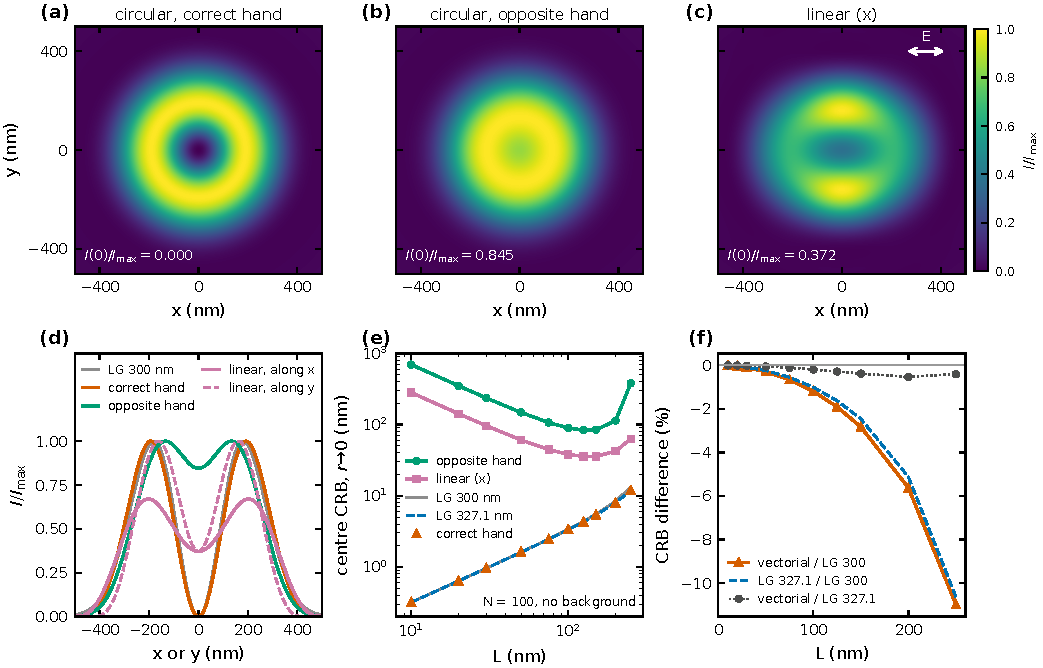
\includegraphics[width=\textwidth]{figures/fig2_vectorial.pdf}
\caption{Vectorial donut. (a--c)~Focal-plane intensity, normalized to the ring maximum, for
circular polarization of the correct hand, of the opposite hand, and for linear ($x$)
polarization. (d)~Profiles through the zero: the zero depth $I(0)/I_{\max}$ is
\pnum{vectorial_zero_depth_correct}\src{vectorial_zero_depth_correct} for the correct hand,
\pnum{vectorial_zero_depth_wrong_handedness}\src{vectorial_zero_depth_wrong_handedness} for the
opposite hand and \pnum{vectorial_zero_depth_linear}\src{vectorial_zero_depth_linear} for linear
polarization. (e)~Centre CRB ($r\to0$ limit, $N=100$, no background) of the TCP versus $L$; all
vectorial beams are evaluated exactly. (f)~Relative CRB differences: the vectorial donut and
the curvature-matched LG with respect to the LG donut with
$\fwhm=\pnum{fwhm_nm}\src{fwhm_nm}$\,nm, and (grey) the vectorial donut with respect to the
curvature-matched LG ($\fwhm=\pnum{vectorial_lg_fwhm_curvature_nm}\src{vectorial_lg_fwhm_curvature_nm}$\,nm),
not to the LG with $\fwhm=\pnum{fwhm_nm}\src{fwhm_nm}$\,nm; the latter CRB ratio is \pnum{crb_vec_over_lgcurv_L150_N100}\src{crb_vec_over_lgcurv_L150_N100} at
$L=150$\,nm.}
\label{fig:vectorial}
\end{figure*}
